\section{System integration and technology stack}

\subsection{Objectives and Framework }
This research achieved parametric coupling of Rhino 9's Grasshopper with JuPedSim, using Grasshopper to represent office floor geometry (polylines as point lists) and initial agent positions(points). A Python script will call JuPedSim's API to map the geometry from Rhino to the input for the JuPedSim scene, utilizing a social force model for microscopic simulations within Rhino. 
\subsection{Technology Stack and Versions}
Rhino 9 (Grasshopper) + Python (3.13, meeting JuPedSim's compatibility requirements);
\\JuPedSim (Julich Pedestrian Simulator) and its Social Force Model; 
\\Data analysis and processing: JupyterLab + Python (Pandas, NumPy, Matplotlib/Seaborn, SQLAlchemy/sqlite3); 
\\Data storage and playback: Each simulation outputs an SQLite database file for offline playback and statistical analysis. 
\subsection{Input and Output Description }
Input: Office geometry (polylines representing contours, doors, corridors, etc.), initial agent positions (Grasshopper point sets), and scene parameters (island table layout, corridor width, number of exits, door widths, etc.). 
\\Output: Each simulation round outputs the raw trajectory data as a SQLite file, while derived metrics such as speeds, congestion events, and other diagnostics are computed from these trajectories for subsequent analysis. Metadata (version, environment, random seed, etc.) are recorded as part of the analysis workflow.
\begin{figure}[h]
    \centering
    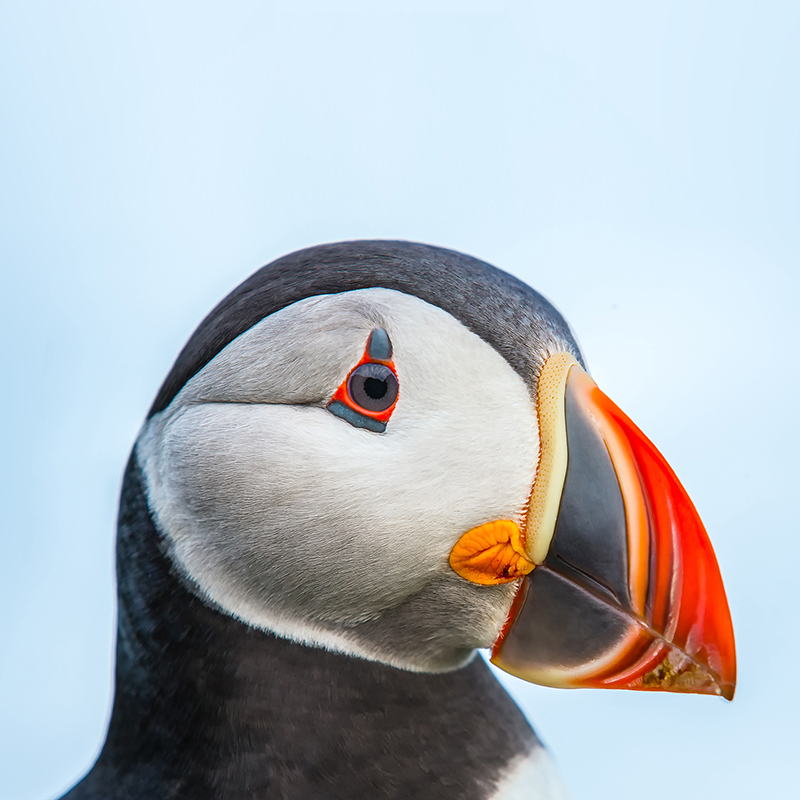
\includegraphics[width=\textwidth]{puffin}
    \caption{Data Pipeline}
    \label{fig:pipeline}
\end{figure}

\section{Experimental design}

\subsection{Prototype Scales}
Small prototype \ref{fig:small}: Focus on the preliminary effects of layout on evacuation paths and times, with rapid iteration through smaller geometric dimensions. To eliminate the influence of multiple corridors, we extended the bottom wall to the leftmost and bottommost sides, keeping only the Main corridor while controlling its width.
\begin{figure}[h]
    \centering
    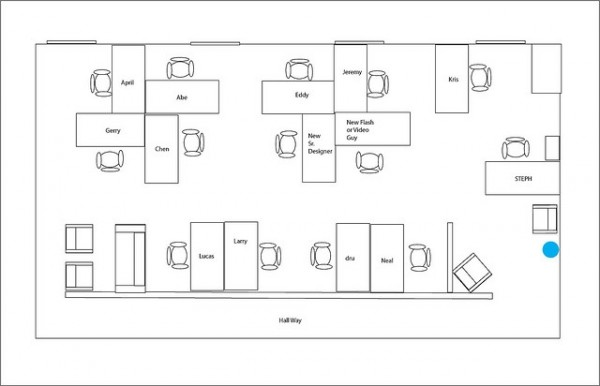
\includegraphics[width=\textwidth]{Small.jpg}
    \caption{Small Prototype}
    \label{fig:small}
\end{figure}
\\Big prototype \ref{fig:big}: Introduce higher-level issues such as door width coupling and multi-room nesting, testing the coupling effects at scales closer to actual office spaces.
\begin{figure}[h]
    \centering
    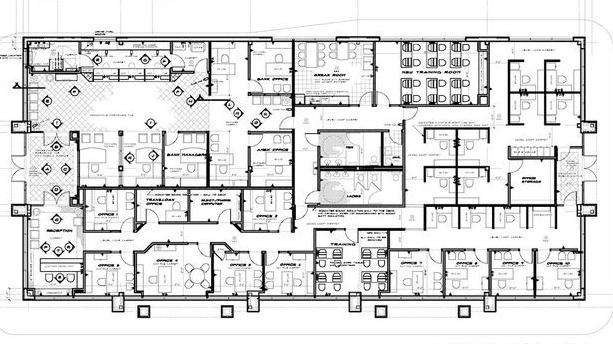
\includegraphics[width=\textwidth]{Big.jpg}
    \caption{Big Prototype}
    \label{fig:big}
\end{figure}

\subsection{Randomness and Replication}
Each parameter configuration is repeated 5 times, with initial positions randomly sampled from a Grasshopper point set to reduce the impact of randomness on the results.

\subsection{Small Prototype Variables}
Island Table Layout \ref{fig:abc}: Three variants A, B, and C represent the internal furniture configuration's representative parameters.
\begin{figure}[h]
    \centering
    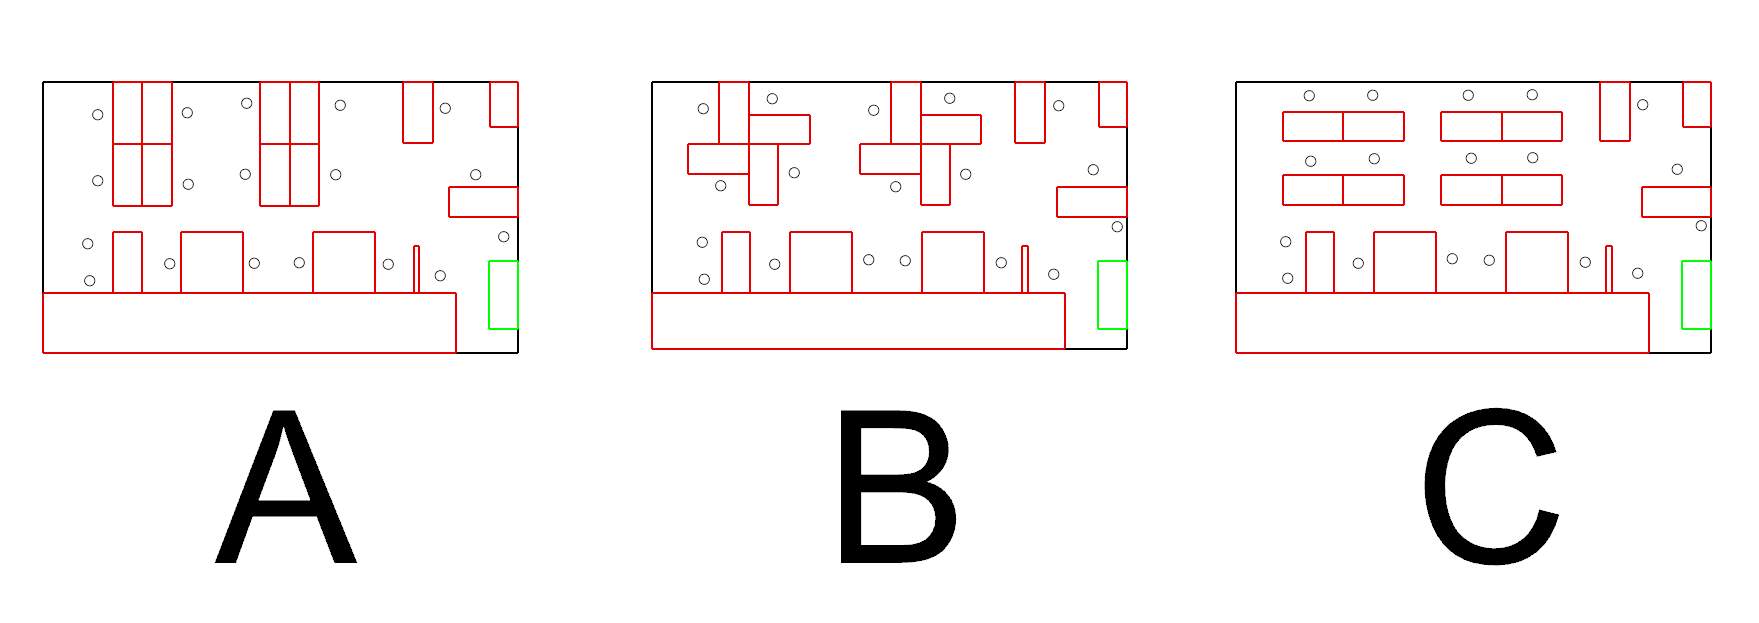
\includegraphics[width=\textwidth]{abc.png}
    \caption{Island Table Layout}
    \label{fig:abc}
\end{figure}

Corridor Width \ref{fig:corridorwidth}: 0.8 m,1.0m, 1.2 m, 1.4m, 1.6 m, 1.8m, 2.0 m, 2.2m, 2.4 m to explore the sensitivity of corridor width on path formation and congestion.
\begin{figure}[h]
    \centering
    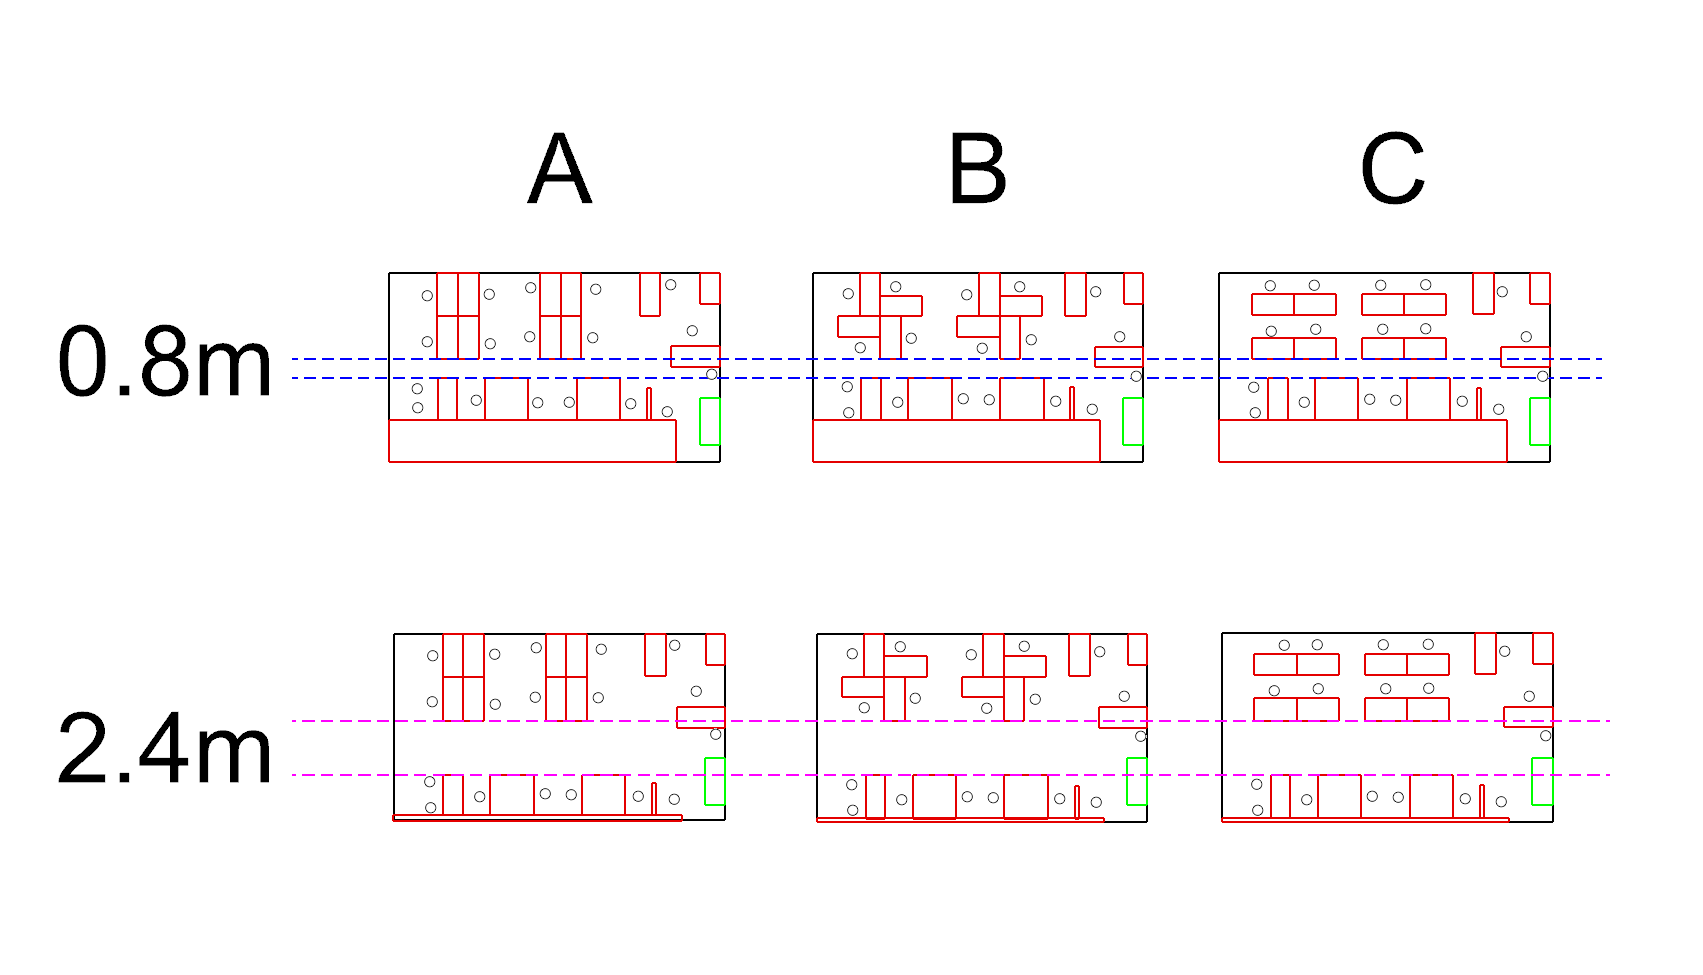
\includegraphics[width=\textwidth]{WidthCompare.png}
    \caption{Corridor Width}
    \label{fig:corridorwidth}
\end{figure}

Exit Configuration \ref{fig:ExitConfiguration}: Single exit and double exit, comparing the impact of different exit quantities on path formation and congestion.
\begin{figure}[h]
    \centering
    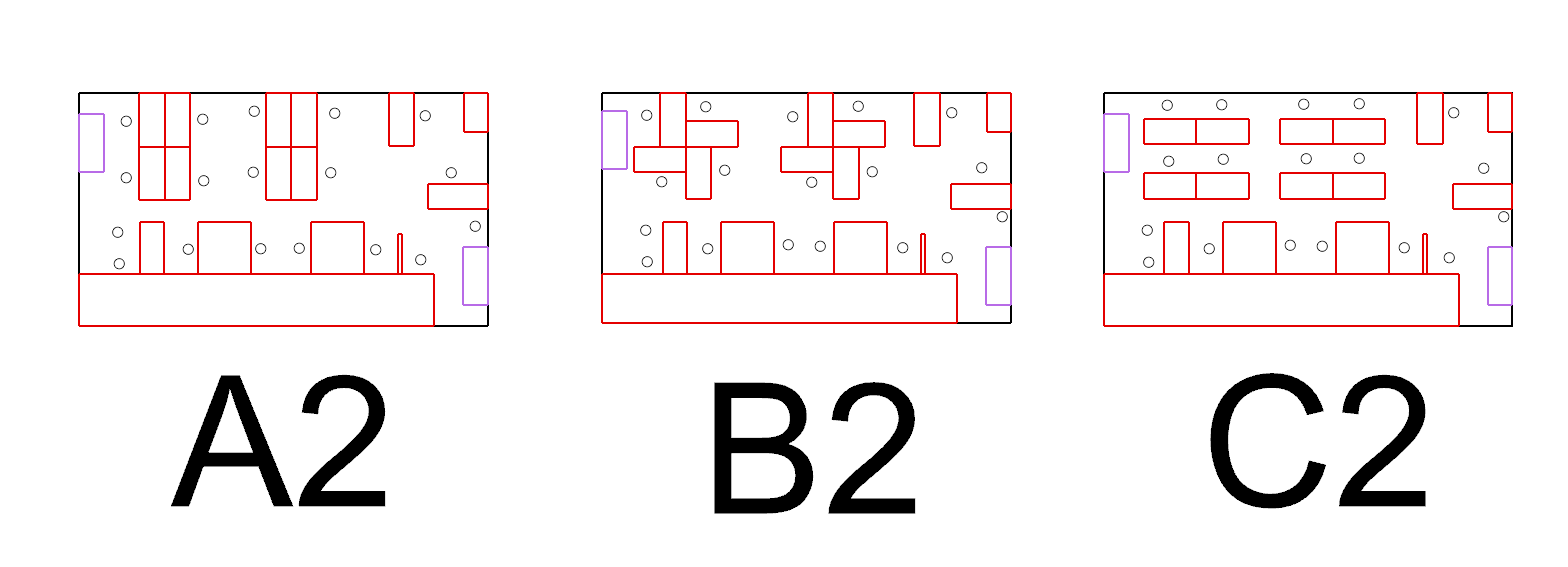
\includegraphics[width=\textwidth]{abc2.png}
    \caption{Exit Configuration}
    \label{fig:ExitConfiguration}
\end{figure}

\subsection{Big Prototype Variables}
We firstly conducted a primitive simulation on the original big prototype. And then we designed two main variable groups based on the primitive simulation results:
\\
Gate width before the exit(the bottleneck) \ref{fig:4ExitsGate}:
\(g\in[1.0,1.6]\text{m}\) is to assess sensitivity of early queuing, discharge rate, and lane merging.
\begin{figure}[h]
    \centering
    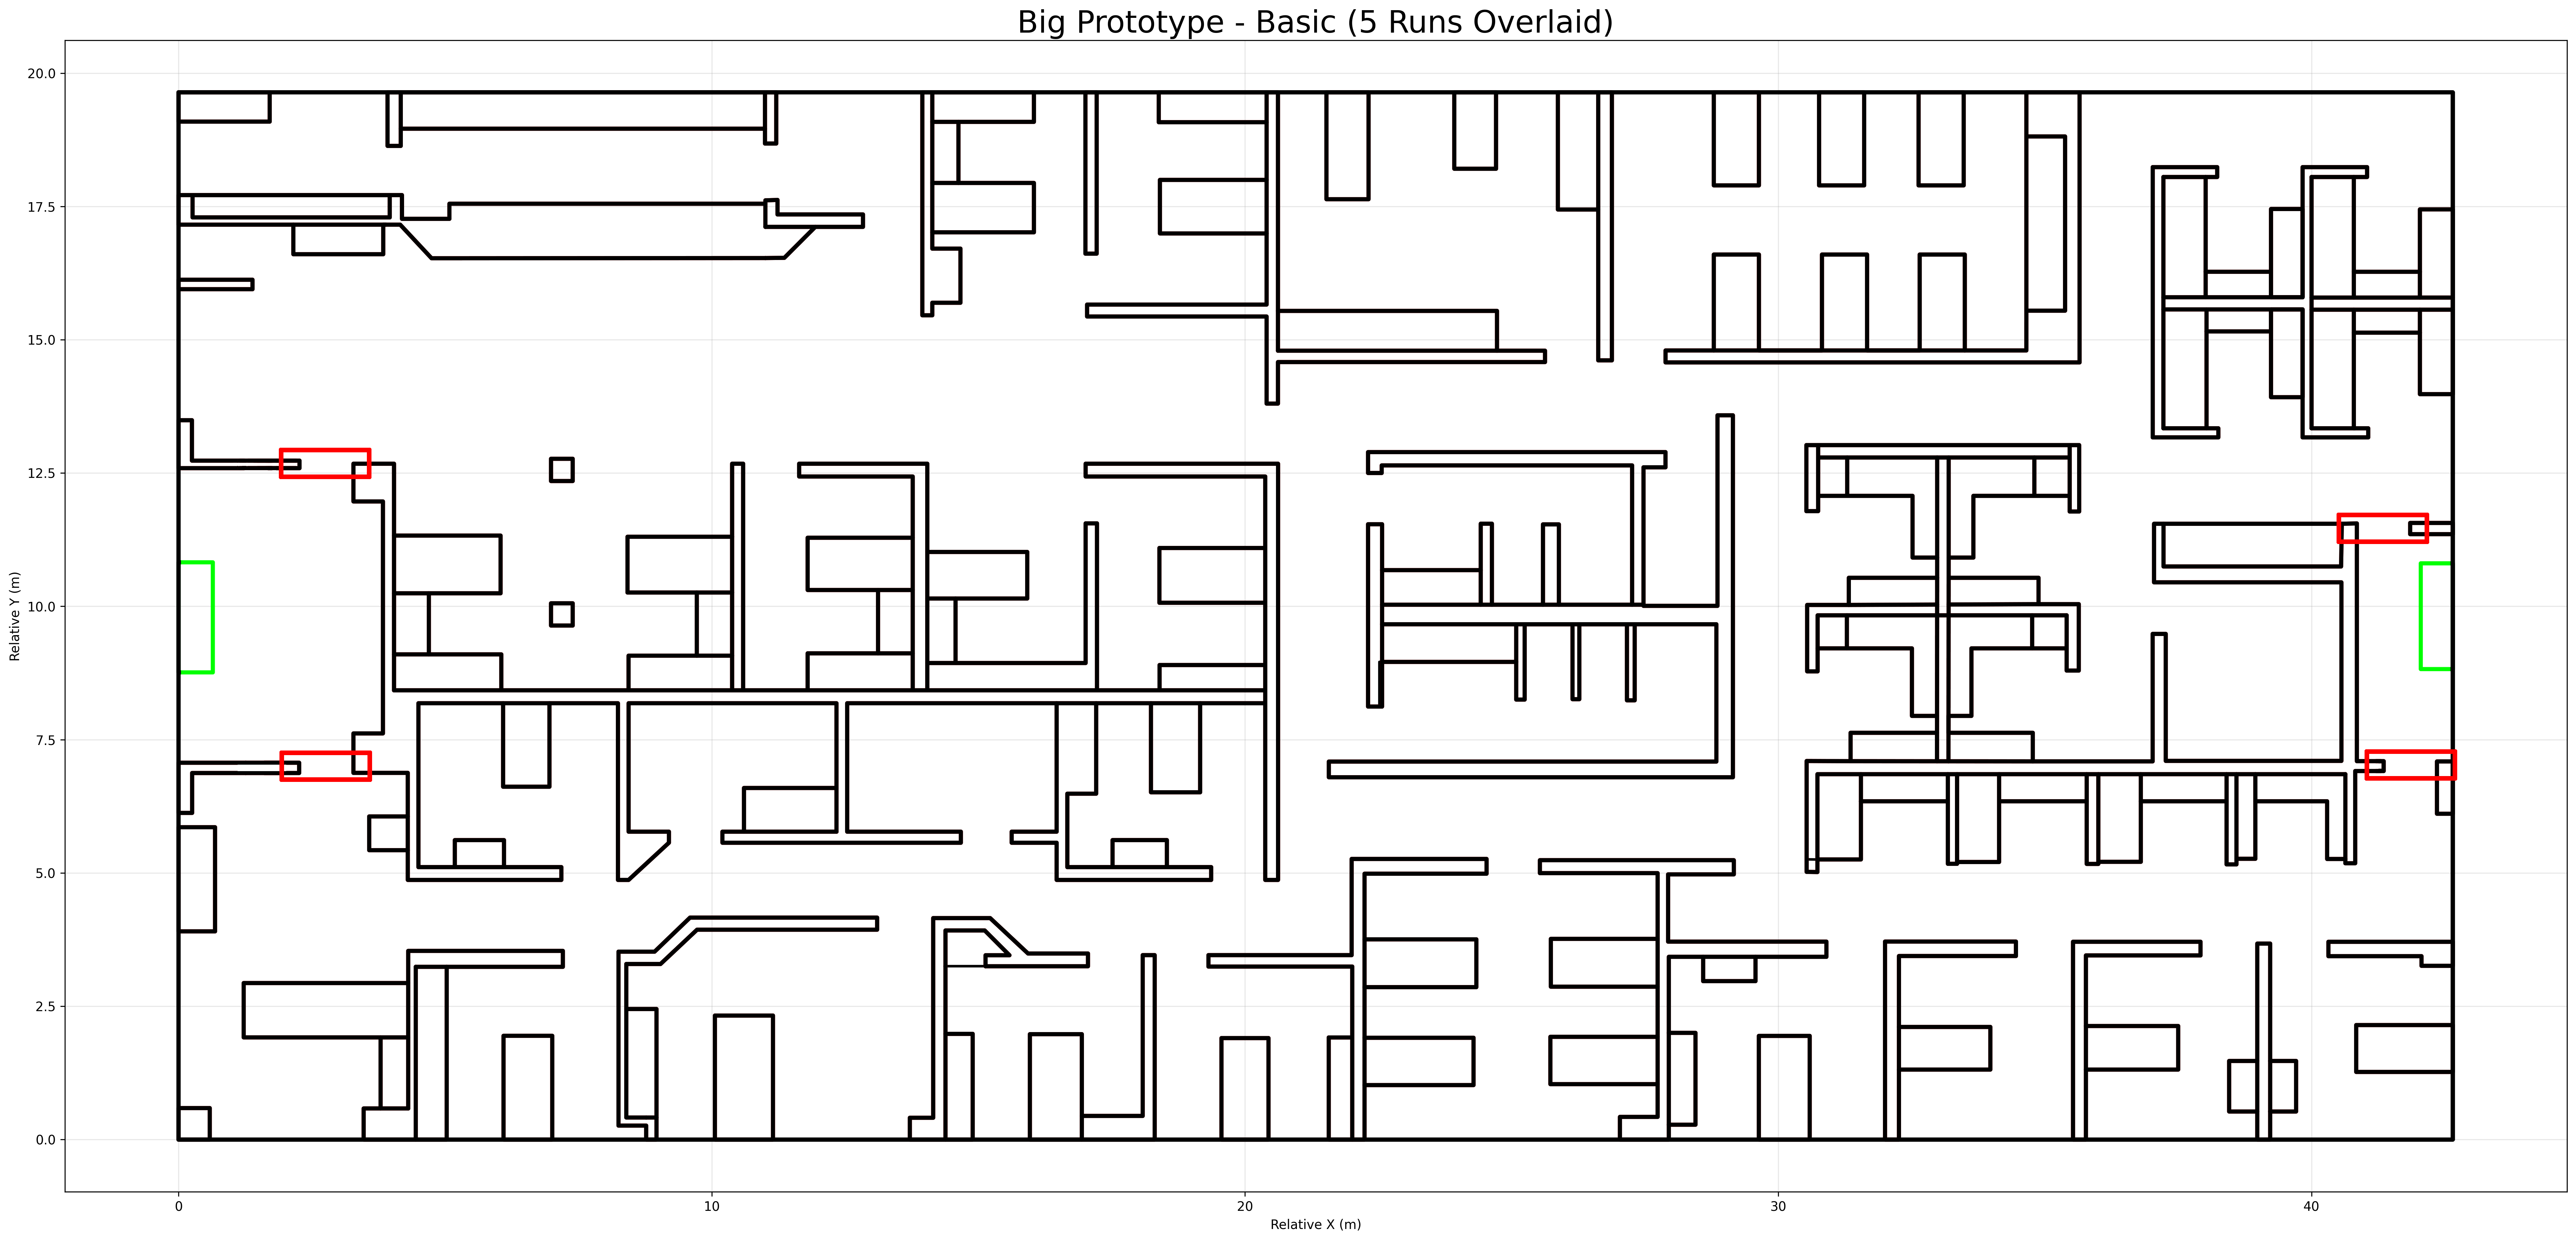
\includegraphics[width=\textwidth]
    {trajectory_overlay_layout_4ExitsGate.png}
    \caption{Change of the gates width before the exits}
    \label{fig:4ExitsGate}
\end{figure}
\\Room-Corridor Coupling: According to the primitive simulation \ref{fig:bigprimitive}, with red lines in the figure representing agent trajectories from all the five runs, the trajectories show convergence into three main corridor segments: corridor a (upper), corridor b (lower-left), and corridor c (lower-right). To quantify the combined effects of "room entrance(blue) and corridor gate(red) width" on the flow distribution and congestion of these main passages, we conducted a full factorial cross-experiment using room door width and corridor gate width entering a/b/c as core independent variables: room door width and gate width in range of {1.0, 1.2, 1.4, 1.6}m. For each combination, we evaluated its impact on early queuing, throughput capacity, and the merging and conflict patterns of the three corridors. 
\begin{figure}[h]
    \centering
    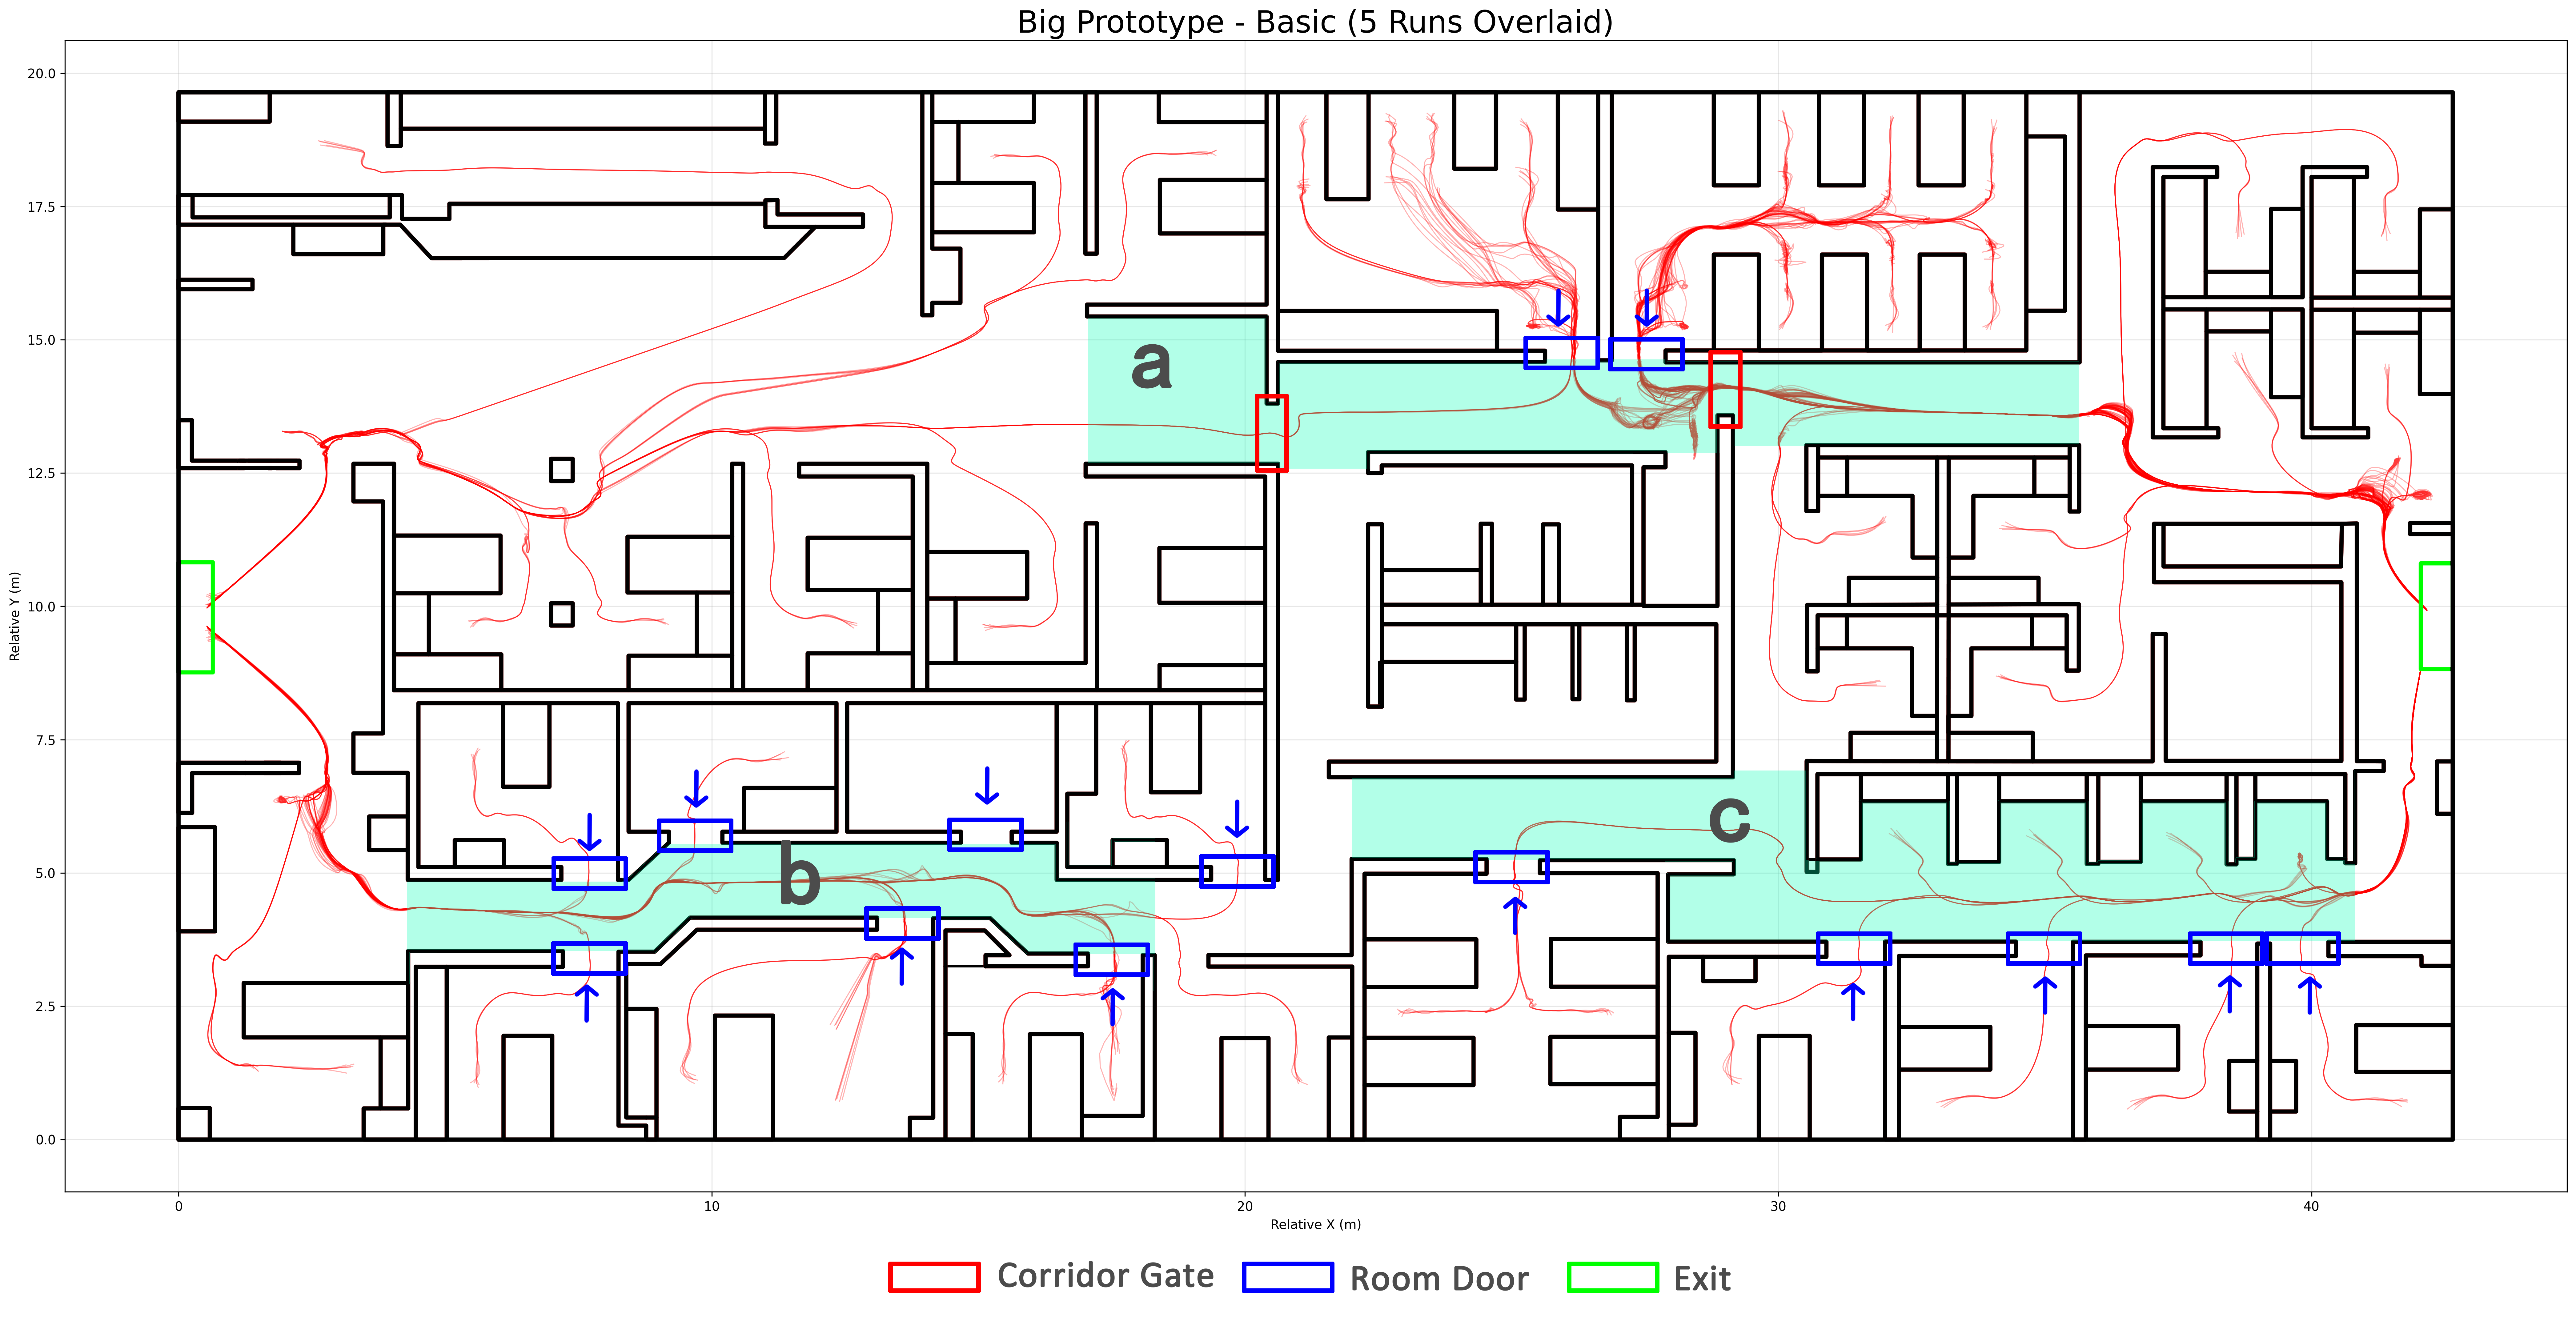
\includegraphics[width=\textwidth]{trajectory_overlay_layout_CorridorAnalysis_Basic.png}
    \caption{Trajectories on the original big prototype and main corridor segments}
    \label{fig:bigprimitive}
\end{figure}

\section{Agents and Model Settings}

This section focuses on clearly setting and recording the attributes of agents (pedestrians), the initial distribution, and the key parameters of the Social Force Model (SFM) within the JuPedSim framework, ensuring comparability and repeatability between different configurations.

\subsection{Agent Attributes and Initial Conditions}

Initial Agent Quantity and Distribution: The total number of agents is set in the Grasshopper/JuPedSim scene input based on the scale of the scenario, with the initial distribution (Grasshopper point set) controlling the initial quantity and spatial distribution.
\\Initial Position Mapping: The point set of Grasshopper is mapped to the initial coordinates of the agents, ensuring that the randomness of initial positions between different configurations is controllable and that repeated experiments can be replicated.
\\Goals and Behavioral Tendencies: Defaults are uniformly set, but in scenarios with multiple entrances, agents tend to choose the shortest path.

\subsection{Social Force Model Parameters}

Model Framework: The built-in Social Force Model of JuPedSim is used as the core microscopic simulation model.
\\Desired Speed: 0.8 m/s is set as the default value, with sensitivity analysis within a range (e.g., 0.6-1.0 m/s) conducted as needed.
\\Interaction Force Parameters: These include repulsive forces between agents, repulsive forces against obstacles, and response intensity to queuing and group aggregation. The initial settings adopt the official recommended values from JuPedSim.
\\Obstacle Handling and Boundary Conditions: The obstacle force scale is set to 1000 to balance the resistance to obstacles in complex scenarios, preventing excessive suppression of agent movement. Boundary conditions follow the wall and exit definitions in the geometric input of the scene.

\section{Data collection and Analysis}

\subsection{Data Output and Storage}
Each simulation produces an independent SQLite database file, recording agent trajectories, speeds, positions, and scene metadata for easy playback and offline analysis.
\subsection{Data Reading and Processing}
Use JupyterLab and Python to read SQLite files (sqlite3), organizing the data into an analyzable structure (DataFrame), and aggregating and statistics on time steps, agent attributes, congestion indicators, etc.

\subsection{Indicators}
\subsubsection{Primary Indicators}
Total Evacuation Time (TET): The overall comparison of evacuation performance under various configurations, which can be presented by evacuation time tables and line charts.
\\
Path Distribution Characteristics: Visualized through trajectory patterns in speed-trajectory diagrams.
\\
Congestion Hotspot Distribution (Hot Zones/Density): The location and extent of low-speed clustering and congestion areas in speed-trajectory diagrams, which equivalently display congestion hotspots and their migration patterns.
\\
\subsubsection{Secondary Indicators}
Path Formation Patterns: Identification of single-lane and double-lanes flow, lane convergence, bottleneck queuing patterns, and their locations based on the trajectory morphology analysis.
\\
Repeated Interval Fluctuation (Robustness): Line overlap/error band performance across multiple runs under identical parameters, expressed as minimum-maximum ranges or mean ± deviation to indicate fluctuation levels.

\subsection{Results Presentation and Visualization}
This study uses Total Evacuation Time (TET) as the primary evaluation metric. For each parameter level (such as door width, corridor width, and exit configuration), we calculate the mean TET and fluctuation range from multiple independent simulations, and conduct direct comparisons and ranking based on these results. To identify potential threshold effects, we observe slope changes in evacuation time line graphs, record parameter intervals where significant inflection points or plateau segments occur, and select representative parameter points to compare with velocity-trajectory diagrams to explain the mechanistic differences in "convergence-merging-queuing" patterns as parameters vary. To ensure the stability of conclusions, each parameter combination incorporates randomized agent initial positions with five repeated experiments.